As mentioned in \cref{sec:arkani-hamed-dimop} in the \gls{add} model, the
fundamental scale of the gravitational interaction, $\md$, is brought down to
the electroweak scale ($\md \approx 1~$TeV). At these energies, due to the large
center of mass energy available at \gls{lhc}, the validity of the predictions of
the \gls{eft} become unreliable. For this reason two different sets of limits
have been calculated, one where the full cross section is used and the other
where it is weighted down by a factor $\md^4/\hat{s}^2$ for events where
$\hat{s} > \md^2$, where $\hat{s}$ is the center of mass energy of the
partons~\cite{LEDWeightFactor}.

% This is implemented in the analysis by first calculating the $\hat{s}$
% distribution for each \gls{sr}

As an illustration of the problem \cref{fig:shat} shows the $\hat{s}$
distribution in the region where $700 < \met < 800$~GeV for the ADD n = 6
model. The straight line indicates the excluded $\md$ value before any weighting
of the events. This figure shows that a fraction of the selected events in the
signal regions have a value of $\hat{s}$ that exceeds the limit of validity of
the effective field theory. The general idea of weighting the events is
therefore introduced. It consists in re-evaluating the limit on $\md$ in a
conservative way, by prescribing that all events with $\hat{s}$ exceeding the
validity limit should only weakly contribute to the limit on $\md$.
% a part of the generated events are in the region where $\hat{s} > \md^2$ where
% the effective field theory predictions are expected to not be reliable.
\cref{fig:vis_sigma_trunc} shows the visible cross section as a
function of the fundamental Planck scale $\md$ in the 700 < $\met$ < 800~GeV
region for the ADD n = 6 model. The solid line is the visible cross section for
all the $\hat{s}$, while in the dashed one a $\md^4/\hat{s}^2$ weighting factor
is applied for events where $\hat{s} > \md^2$, it can be seen that for $\md = 0$
all events get weighted down since $\hat{s} > \md^2 = 0$. The horizontal line is
an hypothesized typical exclusion limit on the visible cross section and it is
not used in the analysis. The intersection point between the dashed line and the
horizontal one, would represent the excluded value on $\md$. The black square is
the nominal $\md$ value of the generated sample.

\begin{figure}[!h]
  \centering
  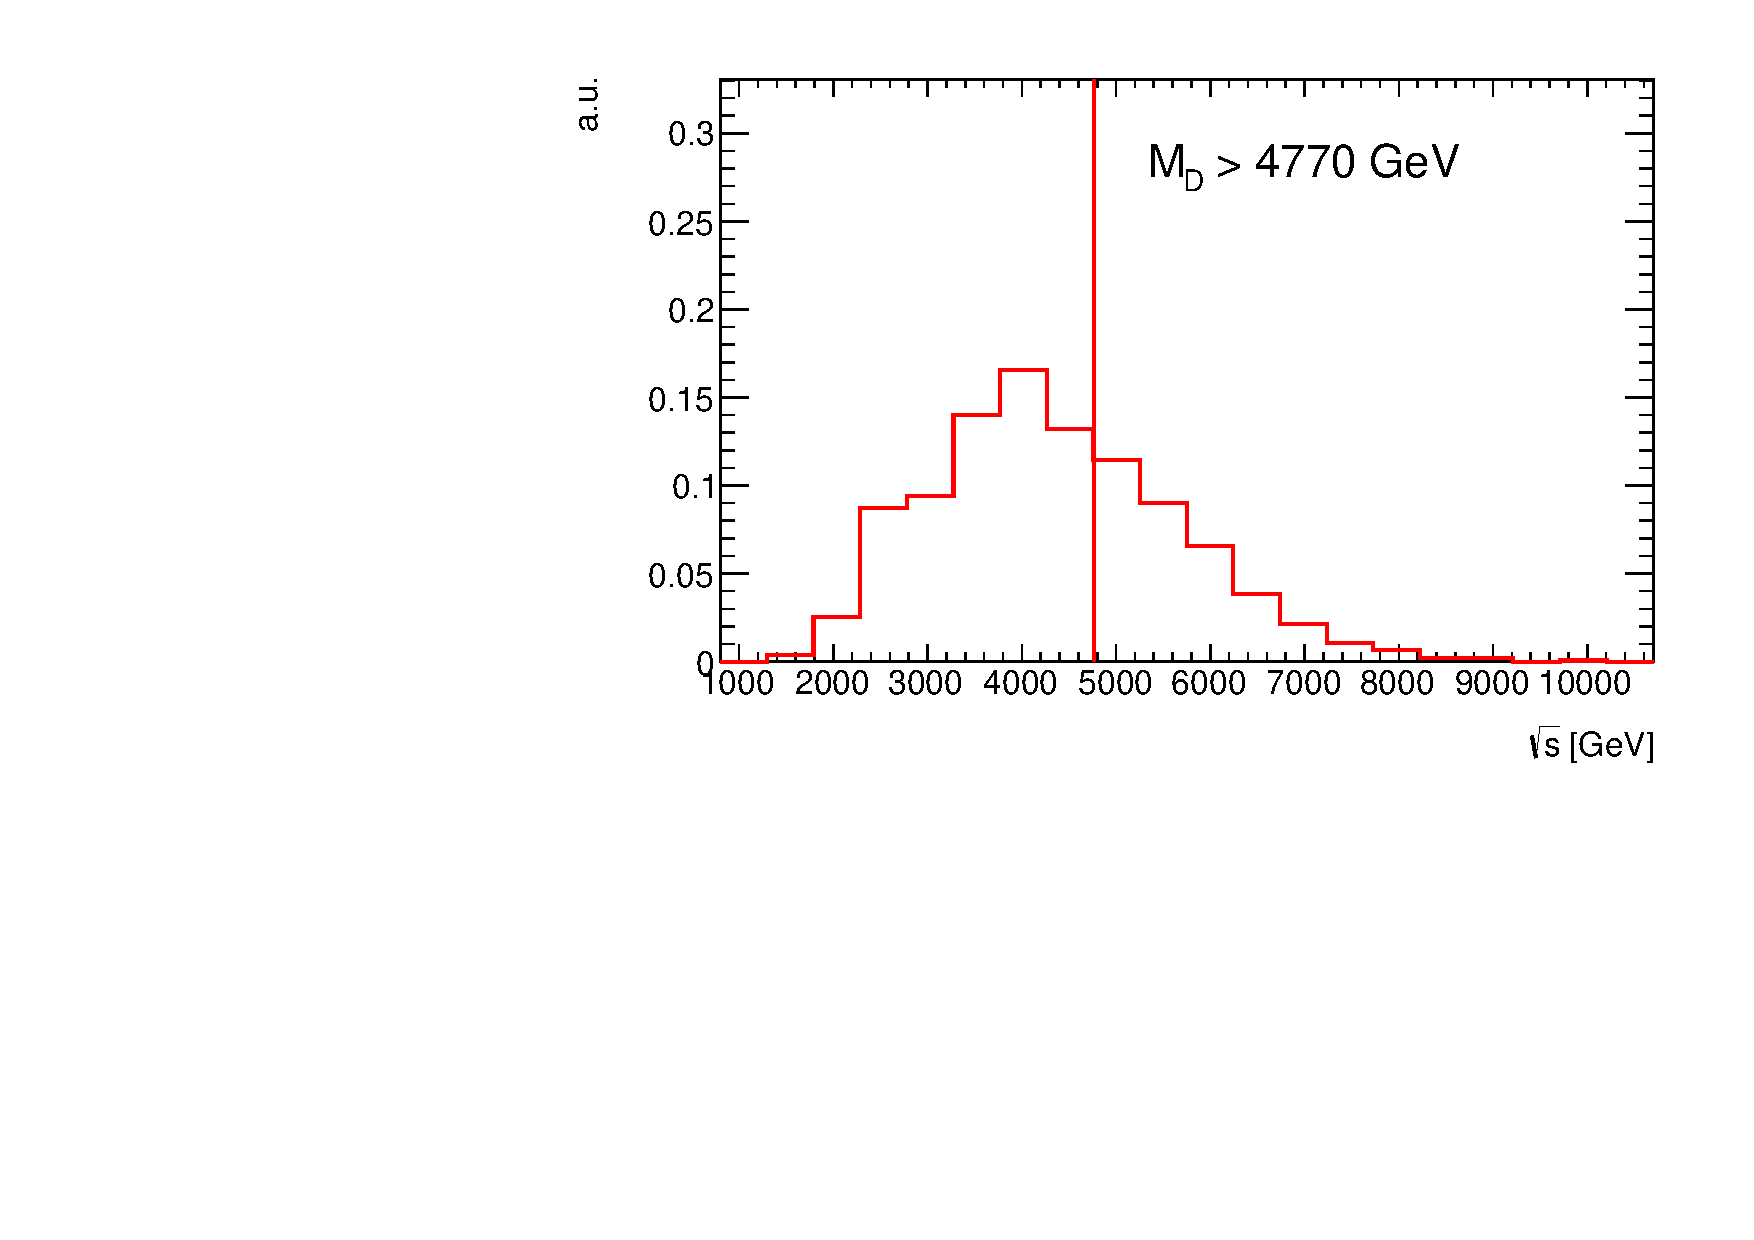
\includegraphics[width=\linewidth]{plot_nD6_SR700}
  \caption{Generated $\hat{s}$ for the signal region where 700 < $\met$ <
    800~GeV for the ADD n = 6 model. A line indicating the value of the excluded
    value of $\md$ is also reported in the figure.}
  \label{fig:shat}
\end{figure}

\begin{figure}[!h]
  \centering
  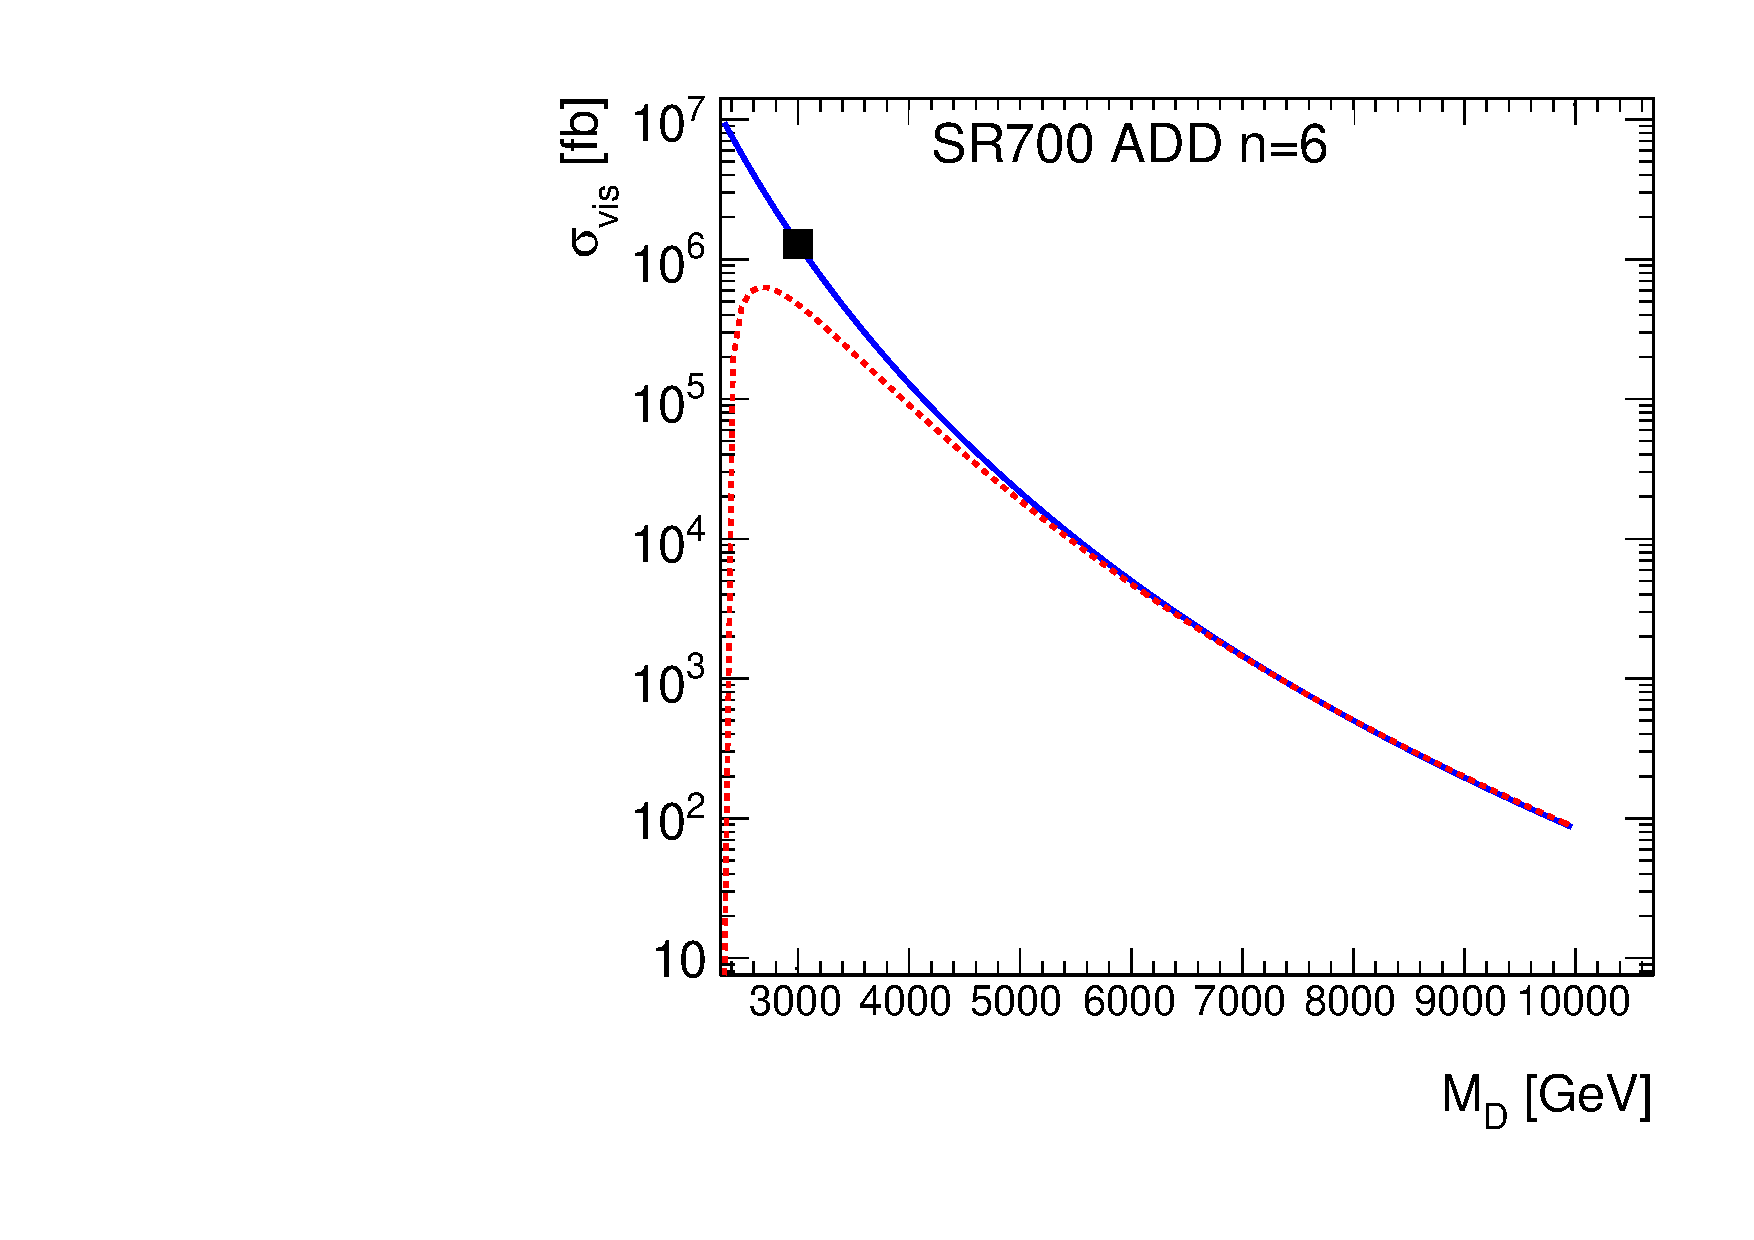
\includegraphics[width=.8\linewidth]{plot_sigma_visible_nD6_SR700}
  \caption{Visible cross section as a function of $\md$ for the signal region
    where 700 < $\met$ < 800~GeV for the ADD n = 6 model. The solid line is the
    visible cross section for all the $\hat{s}$, while in the dashed one a
    $\md^4/\hat{s}^2$ weighting factor is applied for events where
    $\hat{s} > \md^2$. The horizontal line is the upper limit on the production
    cross section if only this region would be considered in the fit. The black
    square is the nominal $\md$ value of the generated sample.}
  \label{fig:vis_sigma_trunc}
\end{figure}
%%% Local Variables:
%%% mode: latex
%%% TeX-master: "../search_for_DM_LED_with_ATLAS"
%%% End:
